\section{Study 3: A Large Preregistered Gain on CLUTRR}
\label{sec:clutrr-external-validation}

The first two studies use synthetic tasks with small models; neither
involves a public, natural-language-like reasoning benchmark.  We therefore
ran a controlled experiment on CLUTRR \cite{sinha2019clutrr}, a public
benchmark of kinship reasoning from generated text.  The question is
narrow: \emph{does training on one set of surface realizations of a
relation pattern improve accuracy on fresh realizations of the same
semantic pattern?}  We report a preregistered pilot (V3) and a
preregistered confirmation on disjoint targets (V4).  The two studies are
never pooled.

\subsection{Task, Unit, and Design}

We freeze CLUTRR Task~1 at relation length three, without distractor facts.
Each example contains a three-edge kinship chain and a query relation drawn
from 23 classes, and entity names are canonicalized by order of appearance.
The semantic identity of an example is the ordered tuple of the target
relation and the three edge relations; sentence order is a surface property
and is not part of the identity.

For every three-sentence source story, we enumerate all six sentence
permutations and group them under one source-group identifier.  A target
pattern is eligible only when it has at least 45 complete source groups.
Its evaluation set contains 200 rows from the first 34 sorted groups (all
six permutations of groups 0--32 and two permutations of group~33); its
training exposure contains 64 rows from the next 11 groups (all six
permutations of groups 34--43 and four of group~44).  Evaluation and
exposure therefore share no source group.

Targets are paired only within the same output relation.  For each model
seed, a frozen SHA-256 bit exposes one pair member in Arm~A and the other
in Arm~B.  Both arms share a 22,720-row base with no target semantics and
append 1,280 target-exposure rows, giving 24,000 training rows per run with
identical label counts.  Initialization, all 30 epoch permutations, tensor
shapes, and dropout RNG trajectories are paired across complementary runs.
The model is a fixed four-layer byte-level Transformer (model dimension
128, four attention heads, feed-forward dimension 512, dropout 0.1),
trained with AdamW at batch size 128 and learning rate $3\times10^{-4}$
under deterministic float32 CPU execution, and evaluated at the fixed
epoch-30 checkpoint after 5,640 updates.  There is no validation selection
or early stopping, and the evaluation manifest is identical across arms
within a block.

\subsection{Estimand and Inference}

For seed $s$, let $\mathbf Z_s^A\in\{0,1\}^{F}$ record which target patterns
are exposed in Arm~A, with
$\mathbf Z_s^B=\mathbf 1-\mathbf Z_s^A$.  For target $f$,
$\mathbf Z_{s,f}^{(1)}$ denotes whichever complete arm assignment exposes
$f$, and $\mathbf Z_{s,f}^{(0)}$ is the complementary assignment.  Let
$A_{s,f}(\mathbf z)$ be row-weighted accuracy under complete assignment
$\mathbf z$.  For $S$ frozen seeds and $F$ frozen targets, the sole primary
estimand is
\begin{equation}
\tau
=
\frac{100}{SF}
\sum_{s=1}^{S}\sum_{f=1}^{F}
\left[
A_{s,f}(\mathbf Z_{s,f}^{(1)})
-A_{s,f}(\mathbf Z_{s,f}^{(0)})
\right]
\quad\text{percentage points}.
\label{eq:clutrr-exposure-estimand}
\end{equation}
As in Study~1, this is the average contrast between two complete
complementary curricula; it includes cross-pattern transfer rather than
isolating one pattern's direct effect.

The 95\% interval uses 20,000 hierarchical percentile-bootstrap replicates
that resample model seeds, complete same-label target pairs, and source
groups within each selected pair member, with source-group draws shared
between exposed and unexposed predictions.  The point estimand is the
finite average over the eight frozen seeds and 80 frozen V4 targets.  The
interval treats the observed seeds, pairs, and within-target source groups
as exchangeable draws from their empirical distributions, conditional on
this model, task, eligibility filter, exposure dose, and budget; because
target selection and group allocation were deterministic, it is not
design-based inference for all eligible CLUTRR patterns, stories, relation
lengths, or architectures.  As a post-hoc sensitivity check, an
intercept-only CR1 cluster-robust estimator clusters the 640 seed-pattern
effects by seed and by complete target pair; the two-way cluster standard
error is 2.6187 points, and a conservative $t_7$ interval is
$[17.1469,29.5313]$.  This check does not replace the registered bootstrap
or alter the decision rule.

\begin{table}[t]
\caption{CLUTRR exposure interventions.  V3 and V4 use disjoint target
semantic patterns and are not pooled.}
\label{tab:clutrr-external-validation}
\centering
\scriptsize
\setlength{\tabcolsep}{3pt}
\begin{tabular}{lrrrrL{1.55in}}
\toprule
Study & Pairs & Targets & Runs & Effect (pp) &
95\% CI; registered outcome \\
\midrule
V3 pilot & 20 & 40 & 16 & $+15.338$ &
$[9.877,21.369]$; precision criterion not met \\
V4 confirm. & 40 & 80 & 32 & $+23.339$ &
$[17.750,29.226]$; directional criterion met \\
\bottomrule
\end{tabular}
\end{table}

\subsection{V3: A Positive but Imprecise Pilot}

V3 froze 20 same-label pattern pairs, eight model seeds, and two arms (16
runs).  Its preregistration allowed a positive, negative, or equivalence
conclusion only if the 95\% interval was at most two points wide.  The
observed effect was $+15.3375$ points with interval $[9.8769,21.3693]$:
positive throughout, but 11.4924 points wide, so the registered outcome is
``positive but imprecise.''  We keep that label rather than relabeling the
pilot after seeing a large estimate.  A post-hoc variance diagnosis
attributes 94.40\% of the bootstrap variance to target-pair resampling, and
a calibrated projection shows that the two-point precision target would
need at least 634 independent pairs while only 139 V3-disjoint eligible
pairs remained.  The strict-precision route was closed, and V3 served only
as a pilot for designing V4.

\subsection{V4: Preregistered Confirmation on Fresh Targets}

Before any V4 training outcome existed, we froze a directional design based
only on V3: a design effect of $7.66875$ points (the smaller of half the V3
point estimate and its lower interval endpoint) and a 100,000-draw Monte
Carlo power analysis over one to four 20-pair blocks.  One block had power
0.7440 and failed; two blocks had power 0.9583 with a 95\% Wilson lower
bound of 0.9570 and were selected.  All 80 V4 targets are semantically
disjoint from the V3 targets, and the success criterion required
$\tau\geq1$ point with the two-sided 95\% interval above zero.

All 32 runs reached the fixed checkpoint and passed post-training integrity
checks: finite model and optimizer state, frozen epoch orders, four-way
paired RNG trajectories, prediction ordering, separate-code-path metric
recomputation, and artifact hashes.  The confirmatory effect is $+23.3391$
points, 95\% CI $[17.7498,29.2257]$: the criterion is met.  Both block
estimates were positive ($+25.0109$ and $+21.6672$ points), as were all
eight seed estimates and all 40 pair estimates; 76 of 80 target patterns
were positive.  These sign counts are descriptive and were not additional
tests.  The secondary proper losses move in the same direction
(exposed-minus-unexposed cross entropy $-1.4938$, multiclass Brier score
$-0.4224$, ECE-15 $-0.2018$); they were registered as descriptive and
cannot alter the accuracy-based primary conclusion.

\subsection{Why Do the Effects Differ?}
\label{sec:why-effects-differ}

The three studies span a near-zero Boolean result, a $+1.8$-point internal
gain, and a $+23.3$-point CLUTRR gain.  We treat this range as the main
behavioral finding, not as noise to average away.  A plausible reading,
which we flag as post hoc: exposure buys little when the model already
executes a short reusable rule (the Boolean tasks, where the released
Transformer scores about 93\% on Conjunction and 78--83\% on Majority and
Sparse Disjunction even without exposure); it buys more where withheld
compositions must be inferred from a limited set of neighbors (CLUTRR
trains a small byte-level model from scratch at one relation length and a
modest budget, a regime in which large seen-versus-unseen gaps are
expected).  A large CLUTRR gap is therefore not surprising in itself.  What
the framework adds is that the gap is attributed to a certified semantic
exposure difference under a preregistered, target-disjoint design, rather
than to a surface-form split that may or may not change semantic exposure.
The practical implication is direct: whether semantic exposure matters is
an empirical property of a model, budget, and task family, so a benchmark
that claims semantic novelty should measure the exposure contrast rather
than assume either a large or a negligible effect.  Figure~\ref{fig:forest}
places the three effects on one axis.

\begin{figure}[t]
\centering
\scriptsize
\definecolor{fblue}{RGB}{46,111,167}
\definecolor{forange}{RGB}{217,142,43}
\definecolor{fgray}{RGB}{107,114,128}
\definecolor{fdark}{RGB}{75,85,99}
\definecolor{fink}{RGB}{43,47,54}
\begin{tikzpicture}[x=1cm, y=0.62cm, font=\scriptsize]
  % study bands: near-zero studies vs large-effect studies
  \fill[fdark!14] (0.8,-0.35) rectangle (9.15,3.55);
  \fill[forange!24] (0.8,3.55) rectangle (9.15,5.45);
  \draw[fdark!35, line width=0.4pt] (0.8,3.55) -- (9.15,3.55);
  % vertical grid
  \foreach \x in {0.8,1.6,2.4,3.2,3.9455,6.4005,8.8555} {
    \draw[gray!25, densely dotted] (\x,0) -- (\x,5);
  }
  % zero line
  \draw[fink, line width=0.5pt] (0.8,-0.35) -- (0.8,5.55);
  % confidence intervals and point estimates
  \draw[fdark, line width=1pt] (0.7264,0) -- (0.8352,0);
  \fill[fdark] (0.7896,0) circle (2pt);
  \draw[fdark, line width=1pt] (0.6408,1) -- (0.8624,1);
  \fill[fdark] (0.7488,1) circle (2pt);
  \draw[fdark, line width=1pt] (0.752,2) -- (1.0256,2);
  \fill[fdark] (0.8736,2) circle (2pt);
  \draw[fblue, line width=1pt] (1.976,3) -- (2.5512,3);
  \fill[fblue] (2.2656,3) circle (2pt);
  \draw[forange!55, line width=1pt] (3.9153,4) -- (6.7367,4);
  \draw[forange!55, line width=0.9pt, fill=white]
    (5.2559,4) circle (2pt);
  \draw[forange, line width=1pt] (5.8481,5) -- (8.6654,5);
  \fill[forange] (7.2203,5) circle (2pt);
  % broken horizontal axis
  \draw[fink, line width=0.5pt] (-0.05,-0.55) -- (3.2,-0.55);
  \draw[fink, line width=0.5pt] (3.7,-0.55) -- (9.15,-0.55);
  \draw[fink, line width=0.5pt] (3.28,-0.62) -- (3.42,-0.48);
  \draw[fink, line width=0.5pt] (3.55,-0.62) -- (3.69,-0.48);
  \foreach \x/\v in {0.8/0,1.6/1,2.4/2,3.2/3} {
    \draw[fink, line width=0.5pt] (\x,-0.55) -- (\x,-0.65)
      node[below] {$\v$};
  }
  \foreach \x/\v in {3.9455/10,6.4005/20,8.8555/30} {
    \draw[fink, line width=0.5pt] (\x,-0.55) -- (\x,-0.65)
      node[below] {$\v$};
  }
  \node[below=0.92cm] at (4.6,-0.55)
    {Exposure effect, exposed minus unexposed (percentage points)};
  % row labels
  \node[anchor=east] at (-0.12,0) {Conjunction};
  \node[anchor=east] at (-0.12,1) {Majority};
  \node[anchor=east] at (-0.12,2) {Sparse Disjunction};
  \node[anchor=east] at (-0.12,3) {Internal (6 architectures)};
  \node[anchor=east] at (-0.12,4) {CLUTRR V3 (pilot)};
  \node[anchor=east] at (-0.12,5) {CLUTRR V4 (confirmatory)};
  % values
  \node[anchor=west] at (9.25,0) {$-0.01\ [-0.09,0.04]$};
  \node[anchor=west] at (9.25,1) {$-0.06\ [-0.20,0.08]$};
  \node[anchor=west] at (9.25,2) {$+0.09\ [-0.06,0.28]$};
  \node[anchor=west] at (9.25,3) {$+1.8\ [1.5,2.2]$};
  \node[anchor=west] at (9.25,4) {$+15.3\ [9.9,21.4]$};
  \node[anchor=west] at (9.25,5) {$+23.3\ [17.7,29.2]$};
  % legend, below the axis title
  \node at (1.30,-3.0) {\textcolor{fdark}{$\bullet$}~Boolean ICL};
  \node at (4.05,-3.0) {\textcolor{fblue}{$\bullet$}~Internal study};
  \node at (6.95,-3.0) {\textcolor{forange}{$\bullet$}~CLUTRR};
\end{tikzpicture}
\caption{Exposure effects across the three controlled studies: exposed
minus unexposed accuracy, in percentage points, with 95\% confidence
intervals.  Colors group the studies: dark gray for the Boolean tasks, blue
for the internal six-architecture study, orange for CLUTRR.  Filled circles
are confirmatory estimates; the open circle is the CLUTRR V3 pilot, which
was positive but did not meet its preregistered two-point precision
criterion.  The horizontal axis is broken between 3 and 9 points because
the Boolean and internal effects sit at zero while the CLUTRR effects are
an order of magnitude larger; that gap is the finding, not a scaling
artifact.}
\label{fig:forest}
\end{figure}

Within CLUTRR, pattern-level effects range from \TTwoMin{} to
\TTwoMax{}~pp and are strongly predicted by the unexposed baseline
(Spearman $\rho=\TTwoSpearman{}$); the median normalized gain is
\TTwoNGMedian{} (Appendix~\ref{tmlrs:app:clutrr-heterogeneity}).
The same headroom pattern holds in the internal finite-function study
(Spearman $\rho=\TThreeSpearman{}$), where the model is near ceiling and
the median normalized gain is only \TThreeNGMedian{}
(Appendix~\ref{tmlrs:app:internal-heterogeneity}).
In a further exploratory (not preregistered) CLUTRR experiment,
same-semantic exposure changes accuracy by \TSixSemGain{}~pp, versus
\TSixDecoyGain{}~pp for relation-matched decoys sharing at least two edge
types; the direct contrast is \TSixSemDecoyGain{}~pp
(95\% CI [\TSixSemDecoyLo{}, \TSixSemDecoyHi{}];
Appendix~\ref{tmlrs:app:semantic-surface}).
The decoy contrast has a positive pattern-cluster interval, but its
four-seed interval includes zero; a zero decoy effect is not excluded
by the seed-level analysis.

\begin{figure}[t]
\centering
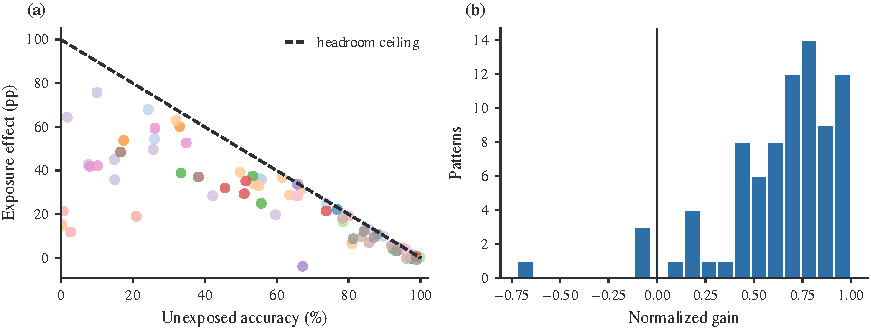
\includegraphics[width=0.98\textwidth]{figures/tmlrs_clutrr_heterogeneity.pdf}
\caption{Exploratory (not preregistered) heterogeneity across the
\TTwoPatterns{} CLUTRR V4 semantic patterns.  In (a), points are colored
by target relation and the dashed line marks the headroom ceiling;
effects are largest when unexposed accuracy leaves more headroom.
Normalized gain (b) remains high for most patterns.}
\label{tmlrs:fig:clutrr-heterogeneity}
\end{figure}

\subsection{What the CLUTRR Result Does and Does Not Say}

The experiment identifies an endpoint effect of randomized complementary
curricula in the frozen CLUTRR setting: the curriculum that exposes a focal
relation composition yields higher focal-pattern accuracy than its paired
alternative, on different source groups and sentence permutations.  This is
a behavioral consequence beyond exact-string reuse, and it supplies the
public-benchmark behavior that the structural audits lack.  It does not
isolate the direct effect of one pattern's exposure from transfer among the
other patterns whose assignments also reverse.

The claim remains deliberately bounded: one CLUTRR task, one relation
length, one architecture, one exposure dose, one optimization budget.  The
result does not show that every form of semantic overlap improves accuracy,
that the model stores a literal lookup table, or that the same effect holds
for unseen relation lengths, family-disjoint reasoning, other
architectures, or natural text.  The near-zero Boolean result stands as a
counterexample to the universal shortcut ``overlap implies memorization.''
The combined evidence supports the weaker and more useful conclusion:
curricula that differ in semantic exposure can have a large behavioral
effect, so benchmark novelty and behavioral exploitation must be measured
separately.
